\chapter{Methodology}\label{chap:Methodology}


\section{Configuration}\label{sec:2-spec}
In this experimental setup, two fundamental sensors are employed to acquire and analyze data.
The Realsense D435i camera, 
known for its high-resolution image capture and depth-sensing capabilities, is utilized for visual data acquisition. 
Complementing the camera is the AWR1843boost mmWave radar, operating in the 77-81GHz frequency range. 
Both sensors are securely housed within a custom 3D-printed enclosure as seen in figure \ref{fig:radar_camera_setup_fig}, 
which not only safeguards them but also minimizes external interference, ensuring the integrity of data acquisition. 
The mmWave radar config that is used is a 77-81GHz chirp, with settings balanced between range and resolution,
collecting data at 20 frames per second.

\begin{figure}[hpbt]
    \centering
    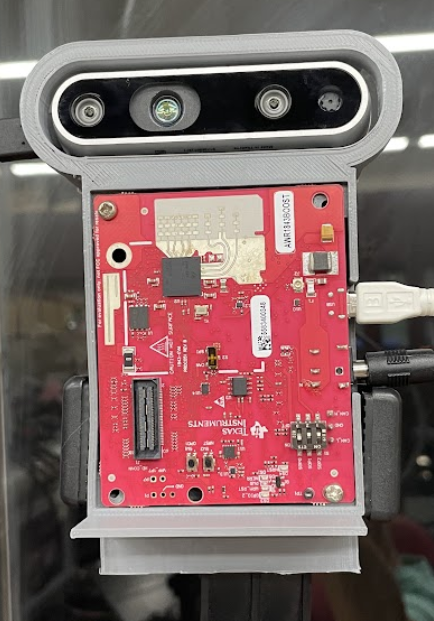
\includegraphics[width=5cm]{Figures/radar_camera_setup.png}%\textwidth
    \caption{Radar camera setup}
    \label{fig:radar_camera_setup_fig}
\end{figure}


\section{Overview}\label{sec:2-overview}
Overview block diagram of the algorithm shown in figure \ref*{fig:kf_update}.
\begin{figure}[hpbt]
    \centering
    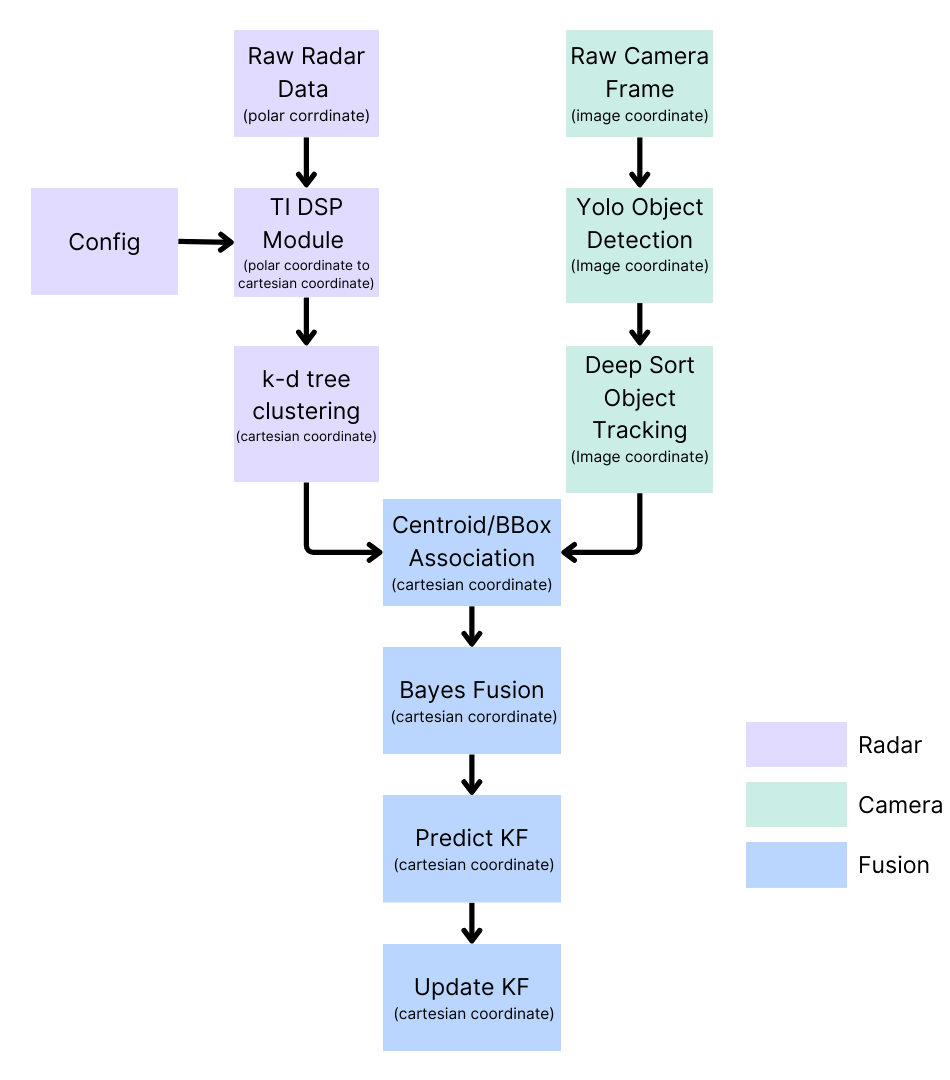
\includegraphics[width=10cm]{Figures/kf_update-modified.png}%\textwidth
    \caption{Radar camera Kalman Filter workflow}
    \label{fig:kf_update}
\end{figure}

\section{Calibration}\label{sec:2-calibration}
\subsection{Camera Intrinsic Calibration}
To accurately map the monocular camera's image coordinates to real-world coordinates, calibration of intrinsic and extrinsic is required.
Using tools provided by ROS \cite{cam_calib} as shown in figure \ref*{fig:camera_calibration}.

\begin{figure}[hpbt]
    \centering
    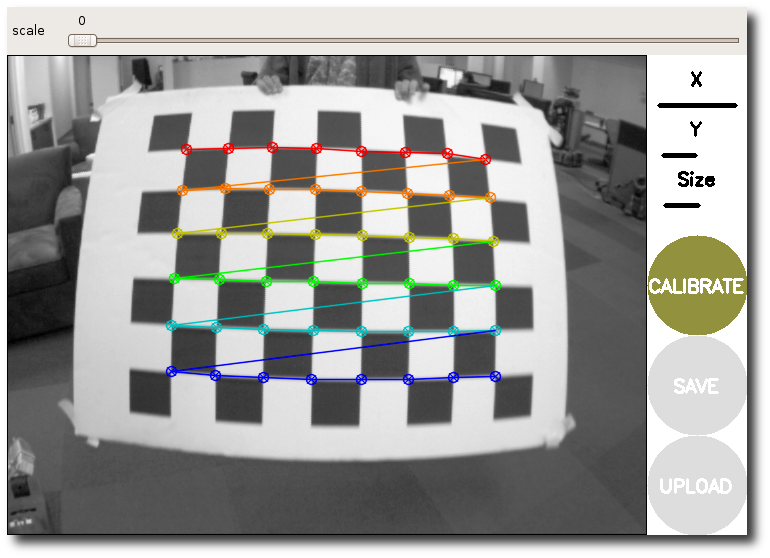
\includegraphics[width=6cm]{Figures/cam_calib.png}%\textwidth
    \caption{Camera extrinsic and intrinsic calibration}
    \label{fig:camera_calibration}
\end{figure}

\subsection{Radar-Camera Transformation Matrix}
While the camera and radar are physically housed as closely as possible, 
as illustrated in Figure \ref{fig:radar_camera_setup_fig}, 
theoretical discrepancies exist.
Accurate fusion of both sensors requires the transformation of their measurements. 
In this scenario, given the challenges in calibrating radar elevation and camera depth, 
a two-dimensional Euclidean space is employed.

\begin{figure}[hpbt]
    \centering
    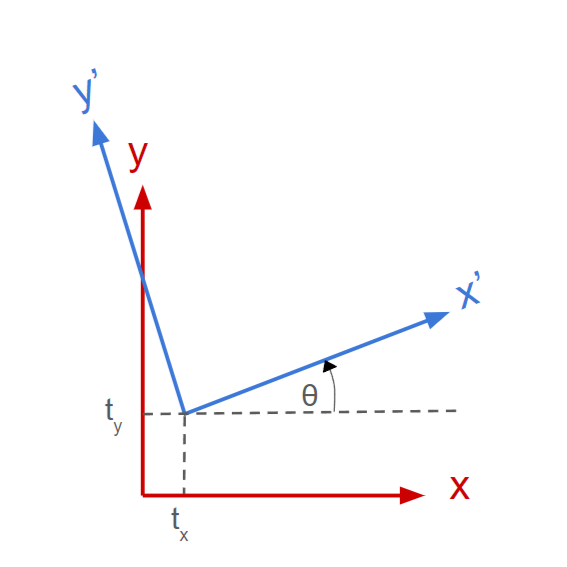
\includegraphics[width=6cm]{Figures/transformation.png}%\textwidth
    \caption{Two rigid body Transformation in 2D coordinate system}
    \label{fig:transformation_figure}
\end{figure}
Let radar coordinates be represented as (x, y), 
and camera coordinates as (x', y'). 
The rotation matrix for the camera with respect to the radar, 
originating from the origin, can be expressed as follows:
\begin{equation}\label{equ:2d_rotation_eq}
    R=
    \begin{bmatrix}
        i_1 & j_1\\
        i_2 & j_2\\
        \end{bmatrix}=
    \begin{bmatrix}
    cos\theta & -sin\theta\\
    sin\theta & cos\theta\\
    \end{bmatrix}
\end{equation}
To relate an arbitrary point in radar coordinates (x, y) to camera coordinates (x', y'), 
the following vector can be employed:
\begin{equation}\label{equ:2d_vector_eq}
    \begin{bmatrix}
        x'\\ 
        y'\\
    \end{bmatrix}=
    \mathbf{t}+x\mathbf{i}+y\mathbf{j}=\mathbf{t}+R
    \begin{bmatrix}
    x\\
    y\\
    \end{bmatrix}
\end{equation}
After encoding the rotation matrix $R$ and the vector, the resulting transformation equation is as follows:
\begin{equation}\label{equ:2d_trans_eq}
    \begin{bmatrix}
        x'\\ 
        y'\\
        1\\
    \end{bmatrix}=
    \begin{bmatrix}
    cos\theta & -sin\theta & t_x\\
    sin\theta & cos\theta & t_y\\
    0 & 0 & 1\\
    \end{bmatrix}
    \begin{bmatrix}
        x\\ 
        y\\
        1\\
    \end{bmatrix}
\end{equation}

\newpage
\subsection{Radar-Camera Data Correlation}
In order to achieve accurate sensor fusion, it is essential to conduct proper calibration of the two sensors. 
For this purpose, a corner reflector is employed (figure \ref*{fig:radar_camera_calibration} \subref{subfig:corner_reflector_fig}), primarily due to its strong radar reflection characteristics(white point in figure \ref*{fig:radar_camera_calibration} \subref{subfig:radar_view_fig}). 
Additionally, it offers the advantage of appearing as a single point in both radar and camera data, effectively reducing ambiguity (figure \ref*{fig:radar_camera_calibration} \subref{subfig:camera_view_fig}).
\subsubsection{Camera to Polar Coordinate Projection}
%Image to Polar Coordinate
The only plane of intersection between the camera and radar in polar coordinates is characterized by theta. 
To integrate the camera data into radar measurements, 
we convert the center of the object detection result into polar coordinates. 
Figure \ref{fig:camera_projection} illustrates the relationship of theta within the camera's plane. 
Equation \ref{equ:img2cart} demonstrates the conversion of pixels to Cartesian coordinates.
\begin{figure}[hpbt]
    \centering
    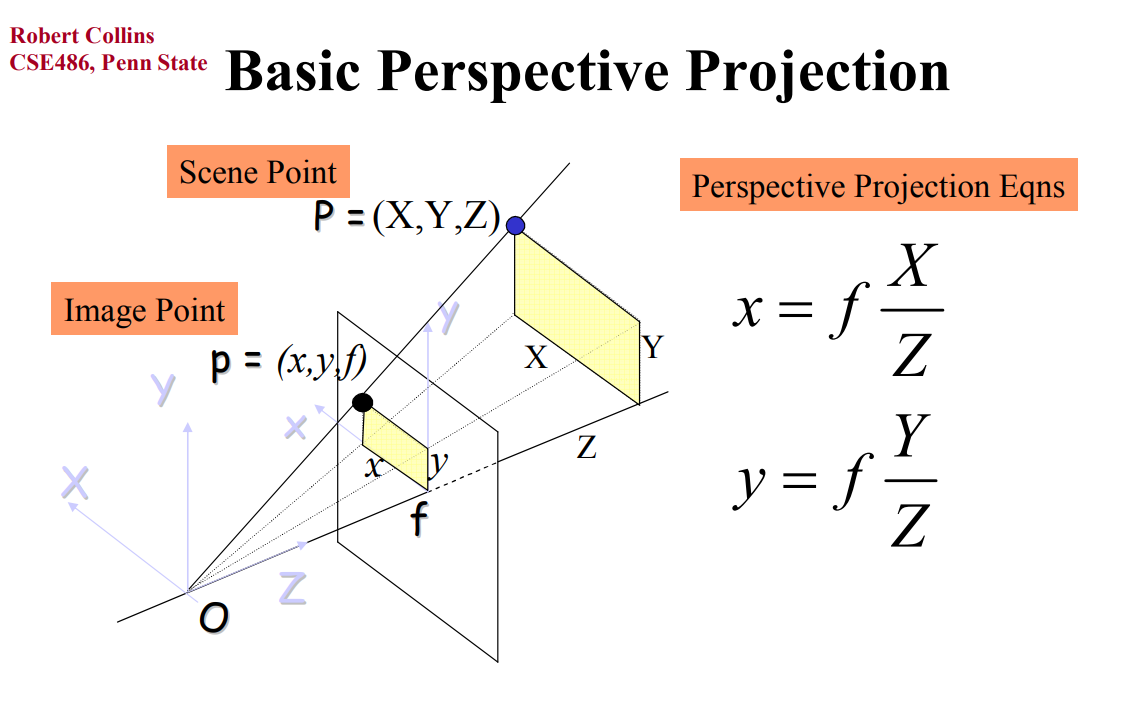
\includegraphics[width=8cm]{Figures/cam_projection.png}%\textwidth
    \caption{Camera to real-world projection}
    \label{fig:camera_projection}
\end{figure}

\begin{equation}\label{equ:img2cart}
u=c_x-\tan^{-1}(\frac{p_x}{p_y})f
\end{equation}
where
\begin{align*}
    c_x &=\text{center of camera image in pixel}\\
    p_x &=\text{x-axis position in cartesian}\\
    p_y &=\text{y-axis position in cartesian}\\
    f &=\text{camera focal length in pixel}\\
    u &=\text{center of Bbox object detection in pixel}
\end{align*}

Since fusion happens in polar coordinates, we need to rearrange the equation to convert camera's horizontal pixel coordinate into theta.
\begin{equation}\label{equ:2_cam_px}
    \theta_{cam}=
    \tan^{-1}(\frac{p_x}{p_y})=
    \frac
    {(c_x-u)}
    {f}
\end{equation}

\subsubsection{Calibrating Camera to Polar Coordinate}

Data points from both radar and camera coordinates can be collected with the corner reflector positioned at various locations.
After data is collected, radar points are associated with image points based on equation \ref*{equ:img2cart}
\begin{figure}[hbpt]
    \centering
    \begin{subfigure}{0.25\linewidth}
        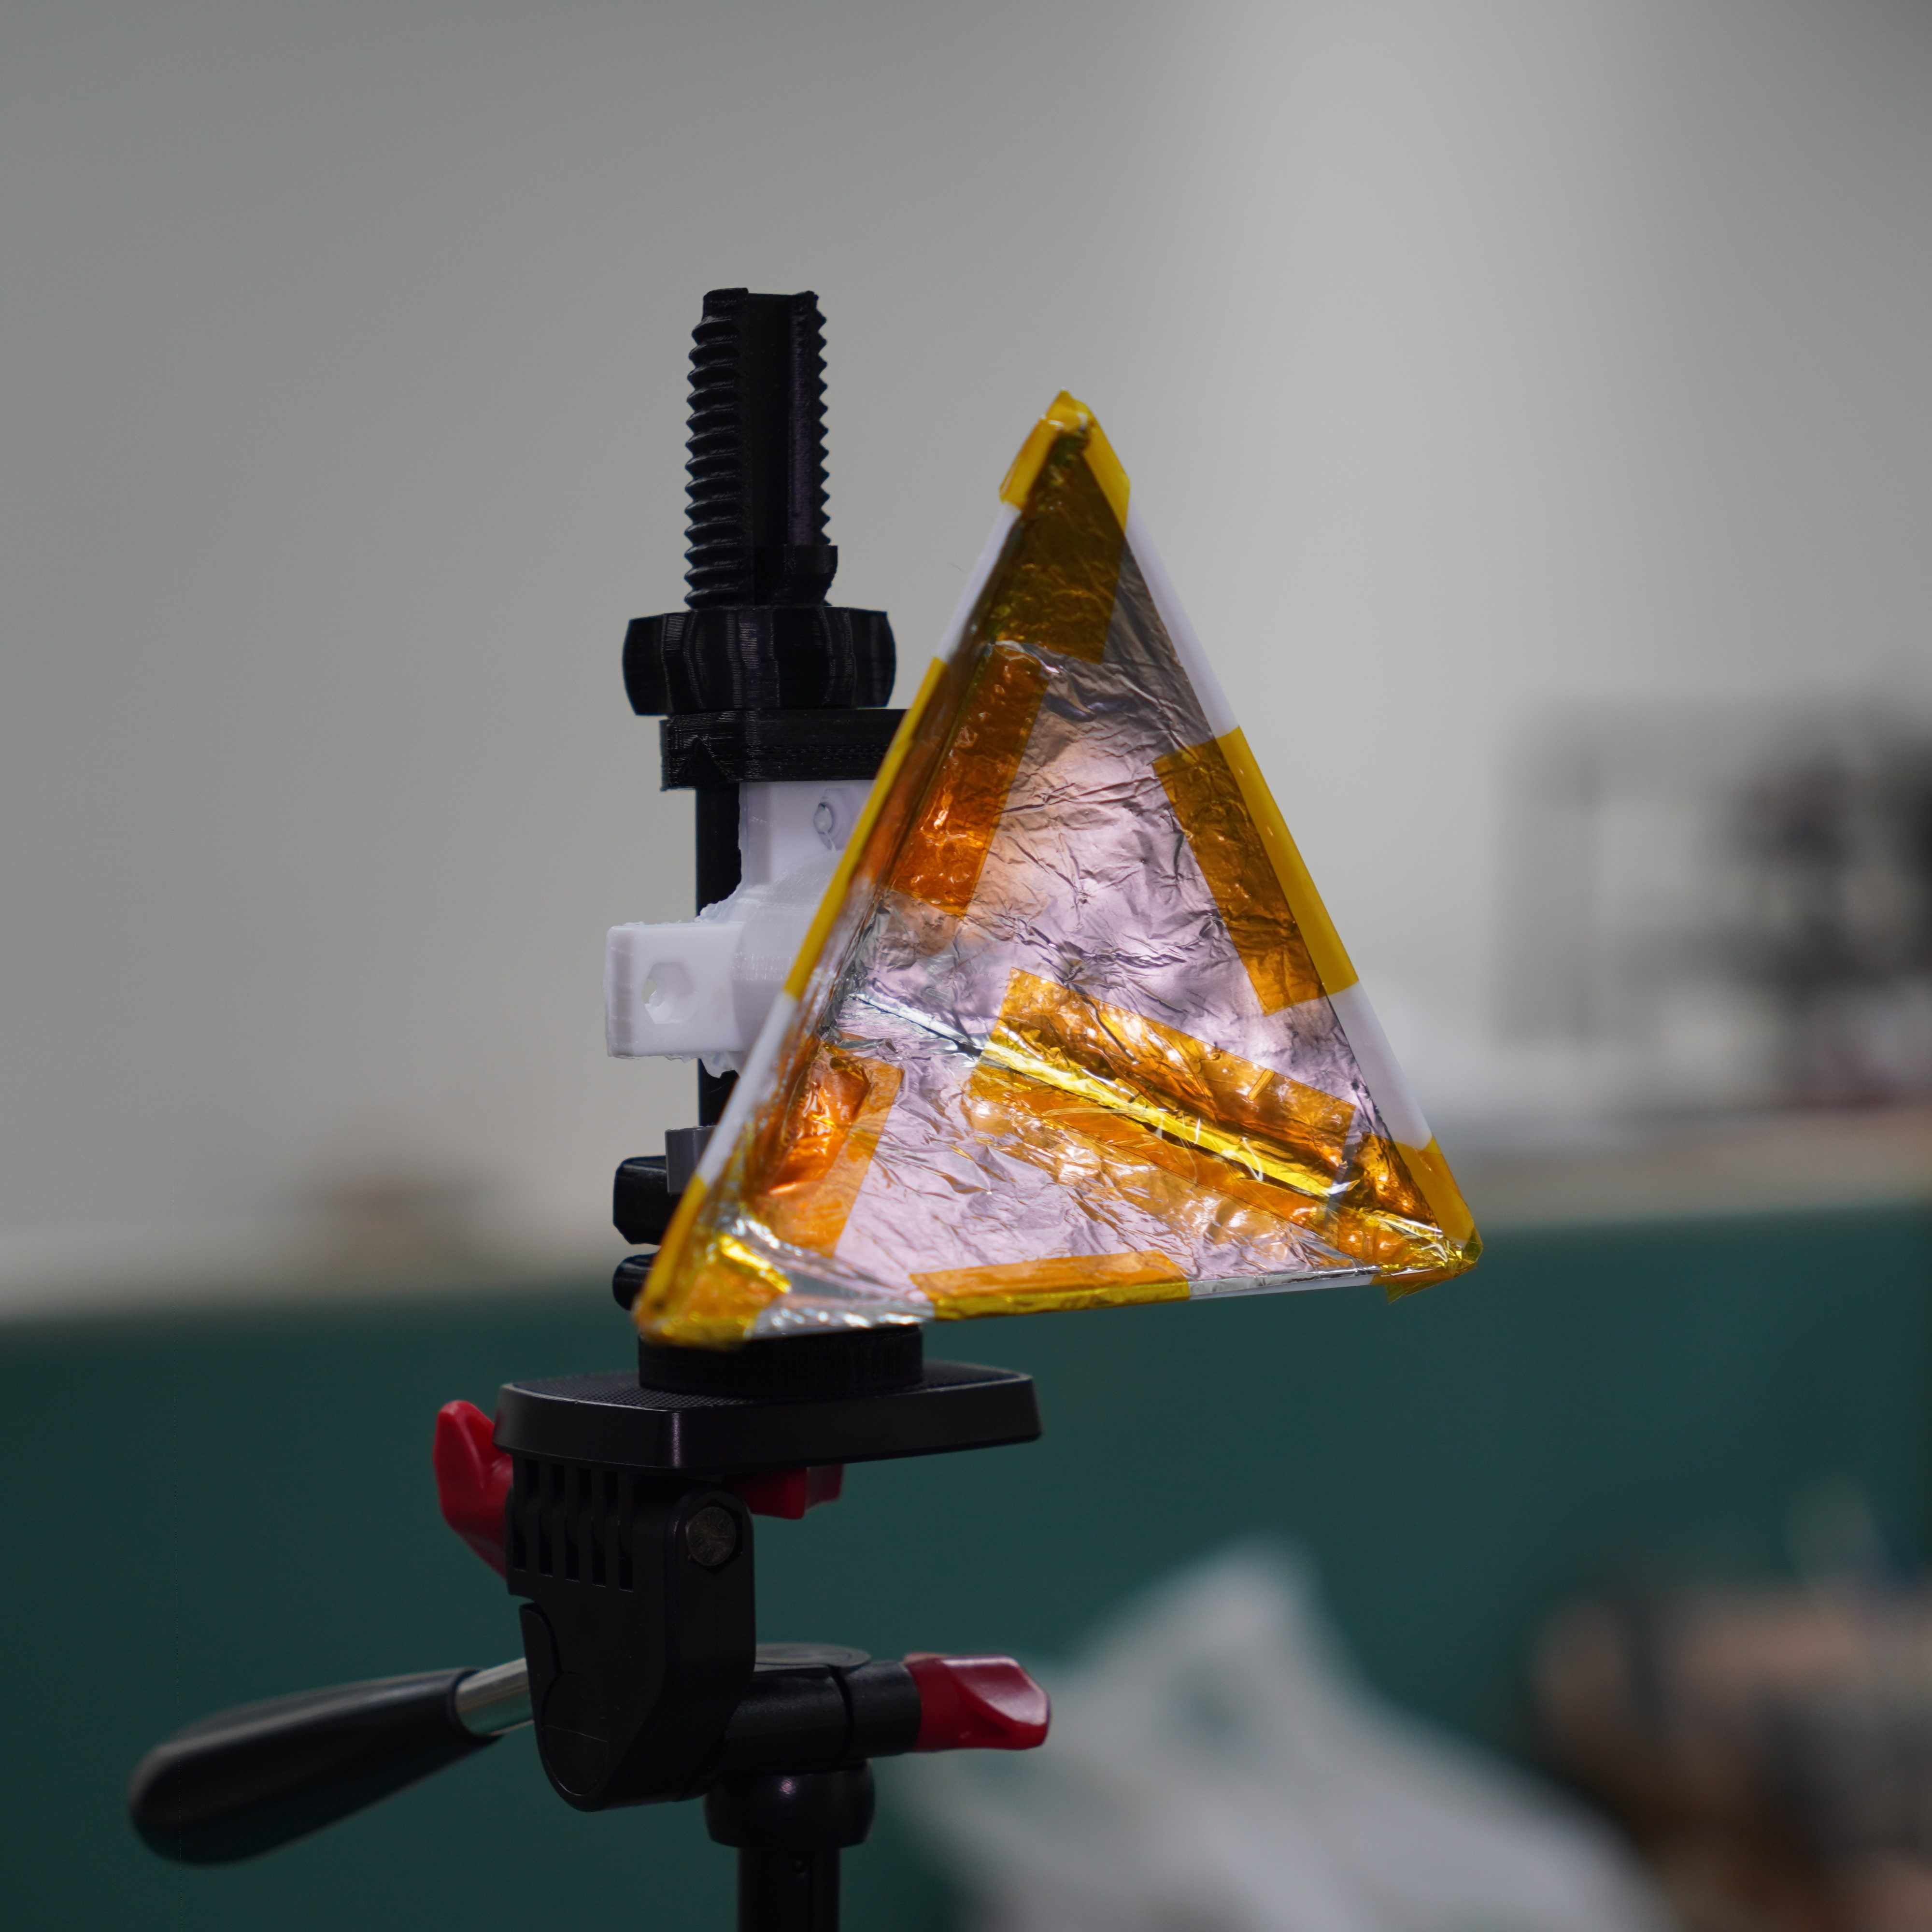
\includegraphics[width=5.5cm]{Figures/corner_reflector.jpg}
        \caption{Radar Corner Reflector}
        \label{subfig:corner_reflector_fig}
    \end{subfigure}
    \hfill
    \begin{subfigure}{0.25\linewidth}
        \centering
        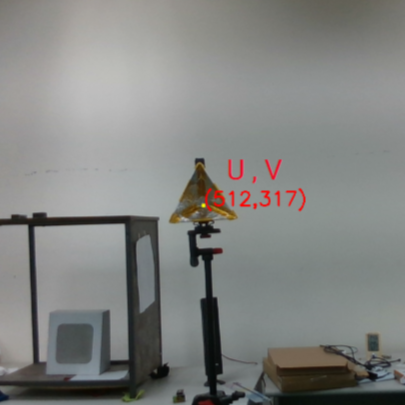
\includegraphics[width=5.5cm]{Figures/camera_corner.png}
        \caption{Camera-corner reflector calibration}
        \label{subfig:camera_view_fig}
    \end{subfigure}
    \hfill
    \begin{subfigure}{0.25\linewidth}
        \centering
        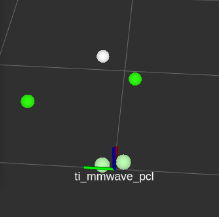
\includegraphics[width=5.5cm]{Figures/radar_corner.png}
        \caption{Radar-corner reflector calibration}
        \label{subfig:radar_view_fig}
    \end{subfigure}

    \caption{Radar camera calibration}
    \label{fig:radar_camera_calibration}
\end{figure}
\begin{table}[h!]
    \begin{center}
      \label{tab:table4}
      \begin{tabular}{l|c} % <-- Alignments: 1st column left, 2nd middle and 3rd right, with vertical lines in between
        \textbf{Method} & \textbf{RMSE} \\% %object detected
        \hline
        Proposed                            & 0.0271 m \\%& 6m 
        \citeauthor{8794186}\cite{8794186}  & 0.025 m \\%
      \end{tabular}
    \end{center}
    \caption{calibration method RMSE compared}
    \label{tab:callib_rmse}
  \end{table}

\begin{figure}[hpbt]
    \centering
    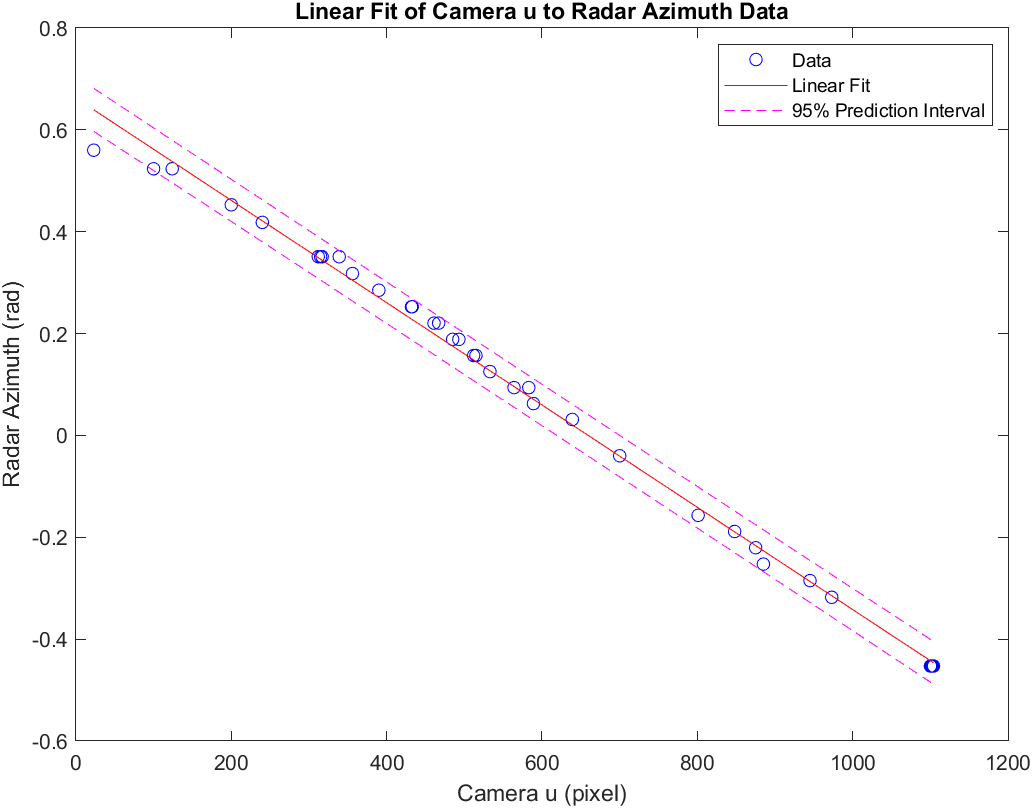
\includegraphics[width=6cm]{Figures/matlab/Linear Fit of Camera u to Radar Azimuth Data.png}%\textwidth
    \caption{Linear Fit of Camera u to Radar Azimuth Data}
    \label{fig:Linear_Fit}
\end{figure}
\newpage
\subsubsection{Generating 3D BBox}
The camera's bounding box detection result is initially expressed in pixels. 
To transform these pixel coordinates into a meaningful real-world 3D bounding box, 
it is essential to acquire the distance of the object, 
a measurement obtained from the radar. 
Once the distance to the object is known, the width of the object can be readily derived using Equation \ref{equ:2_cam_px}.
\begin{figure}[hpbt]
    \centering
    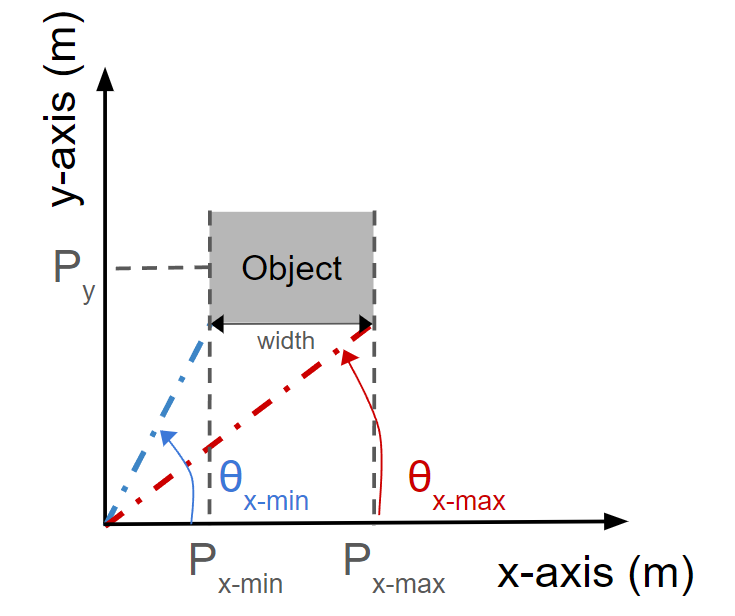
\includegraphics[width=8cm]{Figures/cart_width.png}%\textwidth
    \caption{Object's width to polar coordinates relation}
    \label{fig:cart_width}
\end{figure}
Distance to the object is obtained from range ($\rho$) data from radar:
\begin{equation}\label{equ:2_py_rho}
    P_y=
    \frac
    {cos(\theta)}
    {\rho}
\end{equation}

Where $x_{min}$, $x_{max}$, $x_{min}$, and $x_{max}$ the size of the bbox in pixel obtained from Yolo detection. 
$\theta_{x-max}$ and $\theta_{x-min}$ are obtained from equation \ref{equ:2_cam_px}.
\begin{equation}\label{equ:2_cam_width}
    \begin{split}
    \text{width}&=P_{x-max}-P_{x-min}\\
                &=P_y tan(\theta_{x-max}) - P_y tan(\theta_{x-min})\\
                &=P_y (tan(\theta_{x-max}) - tan(\theta_{x-min}))
    \end{split}
\end{equation}

The same equation can also be applied to derive the height of the detected image. 
\begin{equation}\label{equ:2_cam_height}
    \begin{split}
    \text{height}&=P_{y-max}-P_{y-min}\\
                &=P_y tan(\theta_{y-max}) - P_y tan(\theta_{y-min})\\
                &=P_y (tan(\theta_{y-max}) - tan(\theta_{y-min}))
    \end{split}
\end{equation}






\section{Data Pre-Processing}\label{sec:2-preprocessing}
\subsection{mmWave Radar Data Pre-Processing}\label{sec:2-kd_tree}
Given that radar data is inherently sparse and noisy, its data needed to be filtered.
For this purpose, k-d tree is employed to cluster the pointcloud.
A k-d tree, short for k-dimensional tree, is a hierarchical data structure used for efficient multidimensional data organization and search operations. 
It arranges data points in k-dimensional space, such as spatial coordinates, in a binary tree structure. 

\subsection{Image Data Pre-Processing}\label{sec:2-img_recognition}
\subsubsection{Image Recognition and Tracking}
YOLOv3 is utilized to generate bounding boxes (BBox) and regions of interest (ROI)\cite{redmon2018yolov3}.
Subsequently, DeepSORT is applied for tracking the generated bounding boxes for objects, 
enabling robust and efficient object tracking throughout the analysis\cite{Wojke2017simple}.

\section{Radar-camera Data Association}\label{sec:2-association}
Prior to fusion, radar clusters have to be associated with tracked objects from deepsort.
First, centroids of radar clusters are mapped into image coordinates.
Second, is to find the theoretical error of radar's measurement \cite{8844649}, which is radar's resolution, determined by equation \ref*{equ:angular_resolution}
Finally, if the distance between the calculated radar centroid and the image detection BBox lies within the theoretical boundary
, we can safely assume both measurements belong to the same object of interest.
\begin{equation}\label{equ:angular_resolution}
    \Delta \theta= \frac{c_0}{f_c d N_{RX} N_{TX} \cos(\theta _i)}
\end{equation}
where
\begin{align*}
    f_c & = \text{center frequency} \\
    \lambda & = \text{carrier signal wavelength} \\
    d & =  \lambda/2 \\
    N_{RX} & = \text{Number of receiving antenna}\\
    N_{TX}& = \text{Number of transferring antenna}\\
    \theta _i &= \text{angle of interest}
\end{align*}

\section{Radar-camera Data Synchronization}\label{sec:2-sync}
Given the disparate update rates of radar and camera data, 
coupled with the inherent time required for data processing, 
effective synchronization of measurements becomes crucial. 
Notably, image processing emerges as the most time-intensive step in this synchronization process. 
The algorithm strategically utilizes radar data corresponding to the processed image, storing it for fusion in later stages, 
as depicted in Figure \ref{fig:sync_radar_cam}.
\begin{figure}[hpbt]
    \centering
    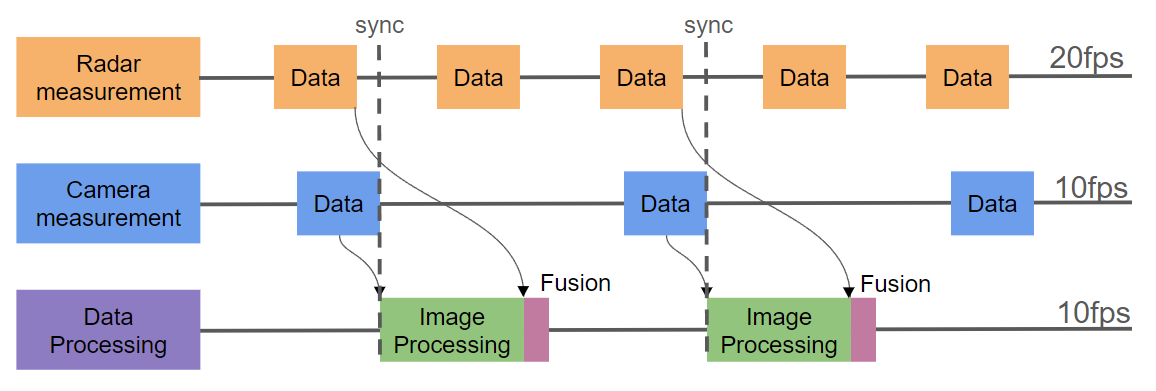
\includegraphics[width=\textwidth]{Figures/syncing.png}%\textwidth
    \caption{Camera and Radar Data Synchronizing}
    \label{fig:sync_radar_cam}
\end{figure}





